\section*{Operações binárias}

\begin{frame}[fragile]{Operações {\it bit} a {\it bit}}

    \begin{itemize}
        \item As operações \textit{bit} a \textit{bit} se comportam da mesma maneira do que suas equivalentes da lógica booleana, considerando o valor \code{cpp}{0}
(zero) como falso e \code{cpp}{1} (um) como verdadeiro

        \item As representações binárias dos operandos devem estar alinhadas (com o mesmo número de dígitos) antes da operação

        \item Se necessário, devem ser adicionados zeros à esquerda

        \item A operação \code{cpp}{&} (e, \textit{and}) resulta em verdadeiro somente quando os ambos \textit{bits} são verdadeiros 

        \item A operação \code{cpp}{|} (ou, \textit{or}) resulta em falso somente quando ambos \textit{bits} são falsos

        \item A operação \code{cpp}{^} (ou exclusivo, \textit{xor}) resulta em falso somente quando ambos \textit{bits} são iguais

        \item A operação \code{cpp}{~} (negação, \textit{not}) é unária e inverte todos os \textit{bits} do operando
    \end{itemize}

\end{frame}

\begin{frame}[fragile]{Visualização das operações {\it bit} a {\it bit}}

    \begin{figure}
        \centering

        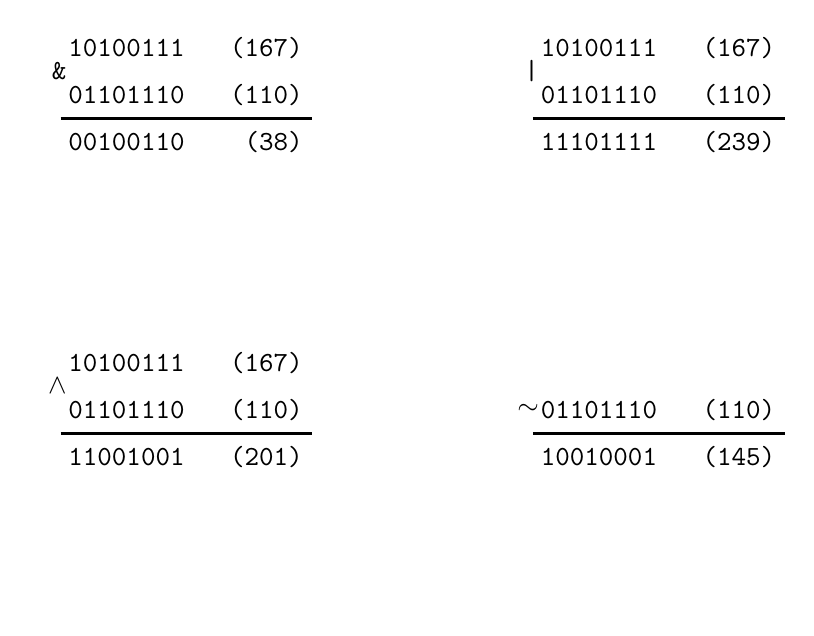
\begin{tikzpicture}
            \begin{scope}
                \node[opacity=0] at (0, 0) { };

                \node[anchor=east] at (2, 3) {  \texttt{10100111} };
                \node[anchor=east] at (3.5, 3) {  \texttt{(167)} };
                \node[anchor=east] at (2, 2.4) {  \texttt{01101110} };
                \node[anchor=east] at (3.5, 2.4) {  \texttt{(110)} };
                \node[anchor=east] at (0.5, 2.7) {  \texttt{\&} };

                \draw[thick] (0.3, 2.1) -- (3.5, 2.1);

                \node[anchor=east] at (2, 1.8) {  \texttt{00100110} };
                \node[anchor=east] at (3.5, 1.8) {  \texttt{(38)} };
            \end{scope}

            \begin{scope}[shift={(6,0)}]
                \node[opacity=0] at (0, 0) { };

                \node[anchor=east] at (2, 3) {  \texttt{10100111} };
                \node[anchor=east] at (3.5, 3) {  \texttt{(167)} };
                \node[anchor=east] at (2, 2.4) {  \texttt{01101110} };
                \node[anchor=east] at (3.5, 2.4) {  \texttt{(110)} };
                \node[anchor=east] at (0.5, 2.7) {  \texttt{|} };

                \draw[thick] (0.3, 2.1) -- (3.5, 2.1);

                \node[anchor=east] at (2, 1.8) {  \texttt{11101111} };
                \node[anchor=east] at (3.5, 1.8) {  \texttt{(239)} };
            \end{scope}

            \begin{scope}[shift={(0,-4)}]
                \node[opacity=0] at (0, 0) { };

                \node[anchor=east] at (2, 3) {  \texttt{10100111} };
                \node[anchor=east] at (3.5, 3) {  \texttt{(167)} };
                \node[anchor=east] at (2, 2.4) {  \texttt{01101110} };
                \node[anchor=east] at (3.5, 2.4) {  \texttt{(110)} };
                \node[anchor=east] at (0.5, 2.7) {  $\land$ };

                \draw[thick] (0.3, 2.1) -- (3.5, 2.1);

                \node[anchor=east] at (2, 1.8) {  \texttt{11001001} };
                \node[anchor=east] at (3.5, 1.8) {  \texttt{(201)} };
            \end{scope}

            \begin{scope}[shift={(6,-4)}]
                \node[opacity=0] at (0, 0) { };

                \node[anchor=east] at (2, 2.4) {  \texttt{01101110} };
                \node[anchor=east] at (3.5, 2.4) {  \texttt{(110)} };
                \node[anchor=east] at (0.5, 2.4) {  $\sim$ };

                \draw[thick] (0.3, 2.1) -- (3.5, 2.1);

                \node[anchor=east] at (2, 1.8) {  \texttt{10010001} };
                \node[anchor=east] at (3.5, 1.8) {  \texttt{(145)} };
            \end{scope}

        \end{tikzpicture}

    \end{figure}

\end{frame}

\begin{frame}[fragile]{Deslocamentos binários}

    \begin{itemize}
        \item O operador \code{cpp}{<<} (deslocamento à esquerda, \textit{left shift}) adiciona o número indicado ($k$) de \textit{bits} iguais a zero à direita do número

        \item A operação equivale à uma multiplicação por $2^k$, de modo que é preciso tomar cuidado com um possível \textit{overflow} 

        \item O operador \code{cpp}{>>} (deslocamento à direita, \textit{right shift}) adiciona o número indicado ($k$) de \textit{bits} iguais a zero à esquerda do número

        \item A mesma quantidade de \textit{bits} à direita são desprezados

        \item Se o sinal é propagado, a operação é denominada deslocamento à direita aritmético; caso contrário, deslocamento à direita binário

        \item No caso do operador aritmético, a operação equivale à uma divisão inteira euclidiana por $2^k$

        \item Em C/C++, o operador \code{cpp}{>>} é aritmético e a divisão inteira (\code{cpp}{/}) não é euclidiana 

    \end{itemize}

\end{frame}

\begin{frame}[fragile]{Exemplos de deslocamentos binários}
    \inputcode{cpp}{codes/shift.cpp}
\end{frame}

\begin{frame}[fragile]{Máscaras binárias}

    \begin{itemize}
        \item Uma máscara binária é um padrão binário que permite a localização, extração ou alteração de determinados \textit{bits} de uma representação binária

        \item A máscara \code{cpp}{(1 << k)} corresponde a todos os \textit{bits} iguais a zero, exceto o $k$-ésimo \textit{bit}, que é igual a um

        \item Esta máscara permite a leitura do $k$-ésimo \textit{bit} de um número através do operador \code{cpp}{&}

        \item Esta mesma máscara permite ligar o $k$-ésimo \textit{bit} de um número através do operador \code{cpp}{|}

        \item A negação desta máscara (isto é, \code{cpp}{~(1 << k)}) permite desligar o $k$-ésimo \textit{bit} de um número por meio do operador \code{cpp}{&}

        \item A máscara \code{cpp}{(1 << k) - 1} permite a extração dos $k$ \textit{bits} menos significativos de um número através do operador \code{cpp}{&}
    \end{itemize}

\end{frame}

\begin{frame}[fragile]{Exemplo de uso de máscaras binárias}
    \inputcode{cpp}{codes/rotate.cpp}
\end{frame}

\begin{frame}[fragile]{{\it Bit} menos significativo}

    \begin{itemize}
        \item O \textit{bit} menos significativo (\textit{least significant bit} - LSB) de um inteiro $n$ pode ser extraído em $O(1)$

        \item Basta fazer a conjunção de $n$ com seu simétrico $-n$

        \item Em C/C++, \code{cpp}{LSB(n) = n & -n}

        \item É possível desligar o LSB com a expressão \code{cpp}{(n & ~LSB(n))}

        \item Porém a expressão \code{cpp}{CLSB(n) = n & (n - 1)} é equivalente, gerando o mesmo resultado com uma sintaxe mais simples e eficiente

        \item A rotina \code{cpp}{CLSB(n)} pode ser usada para contar o número de \textit{bits} ligados de $n$, com complexidade $O(m)$, onde $m$ é o número de \textit{bits} ligados em $n$
    \end{itemize}

\end{frame}

\begin{frame}[fragile]{Exemplo de rotinas com LSB em C++}
    \inputsnippet{cpp}{5}{19}{codes/lsb.cpp}
\end{frame}

\begin{frame}[fragile]{Funções do GCC}

    \begin{itemize}
        \item O GCC oferece uma série de funções de baixo nível para manipulação binária

        \item A função \code{cpp}{__builtin_popcount(x)} retorna o número de \textit{bits} ligados de $x$

        \item A função \code{cpp}{__builtin_clz(x)} retorna o número de zeros à esquerda na representação binária de $x$ (\textit{clz - count leading zeroes})

        \item A função \code{cpp}{__builtin_ctz(x)} o número de zeros à direita na representação binária de $x$ (\textit{ctz - count trailing zeroes})

        \item As duas funções anteriores tem comportamento indefinido se $x$ é igual a zero

        \item A função \code{cpp}{__builtin_ffs(x)} retorna 1 mais o índice do \textit{bit} menos significativo de $x$, ou zero, se $x$ é igual a zero
    \end{itemize}

\end{frame}

\begin{frame}[fragile]{Exemplos de uso das funções do GCC}
    \inputsnippet{cpp}{1}{19}{codes/gcc.cpp}
\end{frame}

